% Offizielle Beispieldatei für beamer-Vorlage aus tubslatex Version 0.3beta2
\documentclass[fleqn,11pt,aspectratio=43]{beamer}

\usepackage[ngerman]{babel}
\usepackage[utf8x]{inputenc}
\usepackage{graphicx}
\usetheme[%
  %nexus,%        Nexus Fonts benutzen
  %lnum,%         Versalziffern verwenden
  %cmyk,%<rgbprint>,          Auswahl des Farbmodells
  blue,%<orange/green/violet> Auswahl des Sekundärfarbklangs
  dark,%<light,medium>        Auswahl der Helligkeit
  %colorhead,%    Farbig hinterlegte Kopfleiste
  %colorfoot,%    Farbig hinterlegt Fußleiste auf Titelseite
  colorblocks,%   Blöcke Farbig hinterlegen
  %nopagenum,%    Keine Seitennumer in Fußzeile
  %nodate,%       Kein Datum in Fußleiste
  tocinheader,%   Inhaltsverzeichnis in Kopfleiste
  %tinytocinheader,% kleines Kopfleisten-Inhaltsverzeichnis
  %widetoc,%      breites Kopfleisten-Inhaltsverzeichnis
  %narrowtoc,%    schmales Kopfleisten-Inhaltsverzeichnis
  %nosubsectionsinheader,%  Keine subsections im Kopfleisten-Inhaltsverzeichnis
  %nologoinfoot,% Kein Logo im Fußbereich darstellen
  ]{tubs}

% Titelseite
\title{Bibtex2HTML}
\subtitle{BibTex zu HTML mit Look \& Feel}
\author{Marcus Stelke, Sven Frank, Frieder Berthold und Alexander Knüppel}
% Titelgrafik, automatisch beschnitten, Weitere Optionen: <scaled/cropx/cropy>
% \titlegraphic[cropped]{\includegraphics{infozentrum.jpg}}
\titlegraphic[scaled]{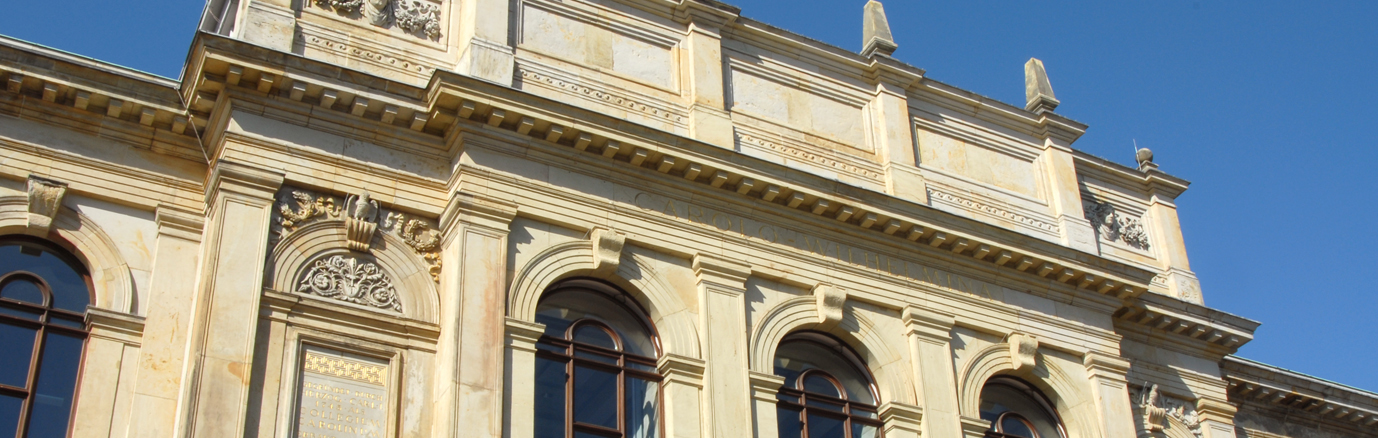
\includegraphics{titlepicture.jpg}}

% Logo, dass auf Titelseiten oben rechts und auf Inthaltsseiten unten rechts
% dargestellt wird. Es wird jeweils automatisch skliert
%\logo{\includegraphics{dummy_institut.pdf}}
\logo{Institut für Softwaretechnik\\und Fahrzeuginformatik}

\begin{document}

\begin{frame}[plain]
\titlepage
\end{frame}

%\begin{frame}{Inhalt}
%\tableofcontents
%\end{frame}


\begin{frame}{Problemstellung}
%TODO Screenshot / Bibtex-File / HTMLcode
\begin{itemize}
\item \textbf{Gegeben}: eine (mehrere) BibTex-File(s)
\item \textbf{Gewünscht}: angepasste und individuelle Darstellung der Inhalte eines BibTex-Files in einem HTML-Dokument
\item \textbf{Problem}: händisch durch Copy \& Paste zu aufwendig \tiny{(und uncool)}
\normalsize
\item \textbf{Lösungsansatz}: Entwerfen einer textuellen DSL mithilfe von Xtext  
\end{itemize}
\end{frame}


\begin{frame}{Workflow}
\begin{figure}
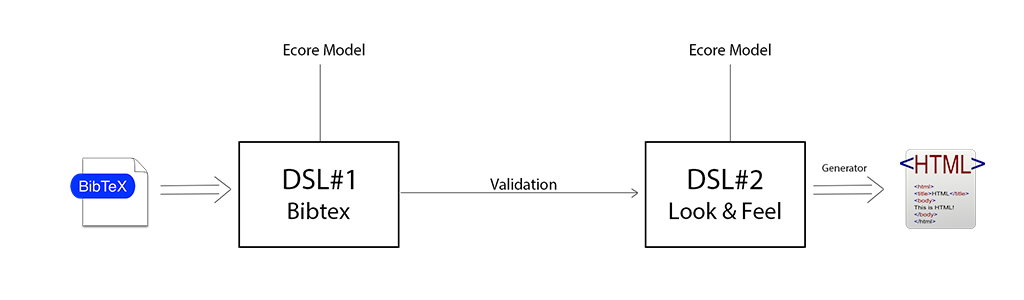
\includegraphics[scale=0.3]{../Images/workflow.png} 
\caption{Workflow}
\end{figure}
\begin{itemize}
\item \textbf{DSL 1 (Bibtex)}:
\begin{itemize}
\item Bildet BibTex-Syntax ab und parst die Einträge zur Weiterverarbeitung
%\item Parst die Einträge zur Weiterverarbeitung
\end{itemize}
\item \textbf{DSL 2 (L\&F)}:
\begin{itemize}
\item Beschreibt, \emph{wie} die HTML-Ausgabe auszusehen hat
%\item Mögliche Funktionalitäten: Diverse Styles von Elementen, Sortierung nach Autor oder Datum,...
\end{itemize}
\end{itemize}
\end{frame}

\begin{frame}{.ecore-Modell: BibTex}
\begin{figure}
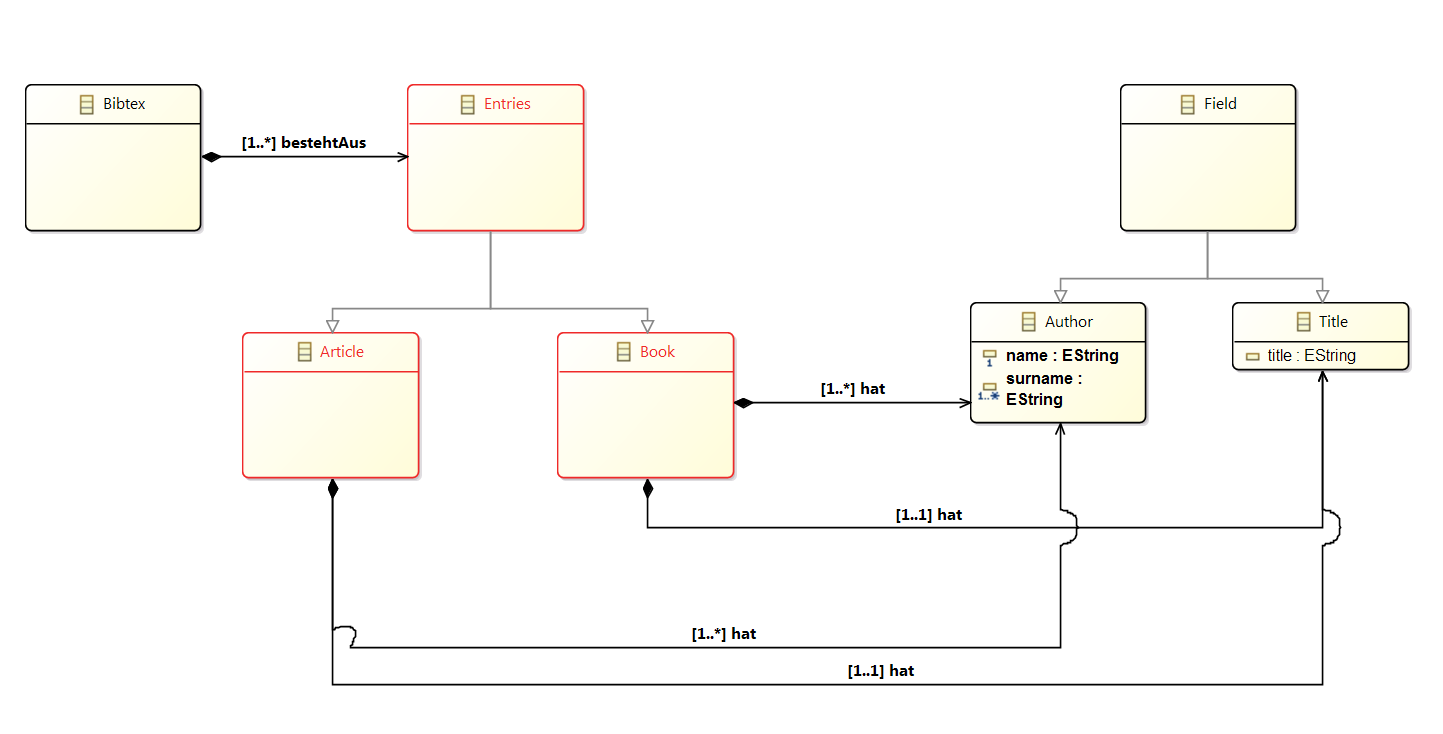
\includegraphics[scale=0.28]{../Images/FirstBibtexEcore.png} 
\caption{BibTex}
\end{figure}  
\end{frame}

\begin{frame}{.ecore-Modell: Output bzw. Look \& Feel}
\begin{figure}
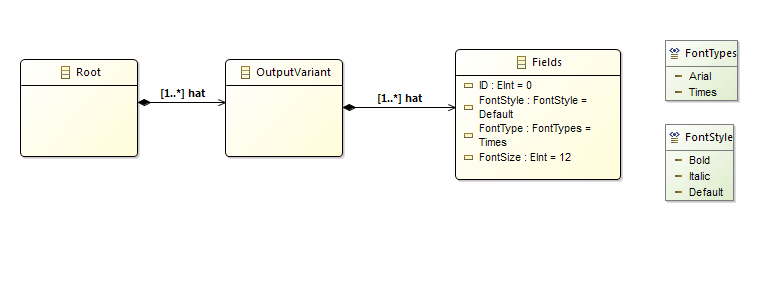
\includegraphics[scale=0.5]{../Images/FirstBibtexToHTMLEcore.png} 
\caption{HTML Generator}
\end{figure}   
\end{frame}



\end{document}
